\section{Structural Overview and Comparison of Welfare Aggregation Criteria}
\label{Sect:Structural_Synthesis}
Sections \ref{Sect:Het_Participants_Unique_Weights}, \ref{Sect:Non-Unique_Weights}, \ref{Sect:Example} and \ref{Sect:Money_Metric_Comparison} develop two distinct paradigms for aggregating individual welfare across heterogeneous pension scheme participants when social planner weights are non-unique or market-consistency is relaxed. In Section \ref{Sect:Non-Unique_Weights}, non-uniqueness of the social planner weights $\alpha$ is handled by evaluating utility-based SCE via Uniform Dominance (Criterion 1), Minimax/Worst-Case SCE (Criterion 2), alongside a preliminary money-metric CES aggregator over raw certainty equivalents $W_{\text{CE}}^k(\alpha; \rho)$ (Criterion 3). Section \ref{Sect:Example} then demonstrates through the closed-form CRRA benchmark that utility-based aggregation and relaxed market consistency based sets $\mathcal{A}_{\kappa}$ suffer from severe structural distortions as risk aversion $\gamma$ increases. Finally, Section \ref{Sect:Money_Metric_Comparison} resolves these distortions by reformulating Criterion 3 around two money-metric ideas that require no Pareto weights. The first one is the Equivalent Contribution at Market Prices ($m_i^k$), aggregated across cohorts via the Atkinson index $\Xi_\rho(k)$ and the second one is the Ex-Post Social Certainty Equivalent $(SCE_{\rho}^{\text{ep}})$ which evaluates intra-state return dispersion via the Equally Distributed Equivalent $e_\rho(\omega)$. The idea of this section is to systematically compare Criterion 1 and Criterion 2 from Section \ref{Sect:Non-Unique_Weights} against the upgraded Criterion 3 from Section \ref{Sect:Money_Metric_Comparison} across four analytical dimensions. First, we will look at the behavior of each criterion when the social planner weights are unique ($\alpha = \alpha^*$). Then, we will analyze what happens to each criterion when market consistency is dropped ($\kappa > 0$), which will be followed by investigating whether the insights of Section \ref{Sect:Het_Participants_Unique_Weights} continue to hold. Finally, we will look at the sensitivity to variation in the degree of risk aversion, especially the case with extreme risk aversion ($\gamma_2 \to \infty$) as in Section \ref{Sect:Example}. It has to be noted that the analysis is organized along two structural comparisons - individual welfare metric (utilitarian vs. money-metric) and interpersonal aggregation device (weight set vs. inequality aversion parameter). We also look at the orthogonal ex-ante vs. ex-post solidarity axis.

\subsection{The Three Aggregation Criteria in Unified Form}
To place the three criteria on a common footing for any candidate risk-sharing rule $k$ and baseline rule (such as the LEL-CE in Sections \ref{Sect:Het_Participants_Unique_Weights} and \ref{Sect:Non-Unique_Weights} and $M$ in Section \ref{Sect:Example}), we summarize their operational definitions in their final form:
\begin{enumerate}
    \item \textbf{Criterion 1: Uniform SCE Dominance (Section \ref{Sect:Non-Unique_Weights})}
    
    Given an admissible set of Pareto weights $\mathcal{A}_\kappa$ induced by relaxing market consistency up to a maximum value transfer of $\kappa W_{i,t}$, rule $k$ uniformly dominates rule $k'$ if and only if:
    \begin{equation}
        SCE_{\alpha}^k \ge SCE_{\alpha}^{k'} \quad \forall \alpha \in \mathcal{A}_\kappa,
    \end{equation}
    where $SCE_{\alpha}^k = G_{\alpha}^{-1}\left(\sum_{i=1}^n \alpha_i \E_t^{\P}[u_{i,t}(W_{i,t+1}^k)]\right)$. Pairwise comparisons are summarized by the utility robustness radius $\hat{\kappa}_u = \sup\{\kappa \ge 0 : SCE_{\alpha}^k \ge SCE_{\alpha}^{k'} \, \forall \alpha \in \mathcal{A}_\kappa\}$, which measures the largest departure from market consistency under which all admissible planners agree on the ranking;
    \item \textbf{Criterion 2: Maxmin/Worst-Case SCE (Section \ref{Sect:Non-Unique_Weights})}
    
    When distributional trade-offs across participants prevents uniform dominance on $\mathcal{A}_\kappa$ ($\kappa > \hat{\kappa}_u$), a social planner evaluates rule $k$ by its worst-case collective value over the admissible weight set:
    \begin{equation}
        \underline{SCE}_{\mathcal{A}_\kappa}^k = \inf_{\alpha \in \mathcal{A}_\kappa} SCE_{\alpha}^k
    \end{equation}
    and ranks rules via the worst-case relative difference $\%\Delta \underline{SCE}_{\mathcal{A}_\kappa}^k = 100 \times (\underline{SCE}_{\mathcal{A}_\kappa}^k - \underline{SCE}_{\mathcal{A}_\kappa}^b)/W_t$;
    \item \textbf{Criterion 3: Money-Metric Aggregation (Section \ref{Sect:Money_Metric_Comparison})}
    
    Rather than aggregating raw certainty equivalents $CE_{i,t}^k / W_{i,t}$ over an unknown weight set $\alpha \in \mathcal{A}$ as in the preliminary specification of Section 6, the upgraded Criterion 3 of Section \ref{Sect:Money_Metric_Comparison} decouples efficiency, preference heterogeneity, and ex-post solidarity through two weight-free money-metric aggregators:
    \begin{itemize}
        \item \textbf{Criterion 3a (Ex-Ante Equivalent-Contribution Index:)}
        
        Each member's welfare is measured by her equivalent contribution at reference state prices, $m_i^k = \min\{\pi_t(X) : \E_t^{\P}[u_{i,t}(X)] \geq \E_t^{\P}[u_{i,t}(W_{i,t+1}^k)]\}$, and aggregated across the scheme via the contribution-weighted Atkinson index:
        \begin{equation}
            \Xi_\rho(k) = \left( \sum_{i=1}^n \frac{W_{i,t}}{W_t} \left( \frac{m_i^k}{W_{i,t}} \right)^{1-\rho} \right)^{\frac{1}{1-\rho}}, \quad \rho \ge 0
        \end{equation}
        Rule $k$ robustly dominates rule $k'$ across all degrees of societal inequality aversion $\rho \ge 0$ if and only if the vector of equivalent-contribution returns $(m_i^k / W_{i,t})_{i=1}^n$ Generalized Lorenz dominates $(m_i^{k'} / W_{i,t})_{i=1}^n$.

        \item \textbf{Criterion 3b (Ex-Post Solidarity Index):}
        
        To evaluate rules that introduce ex-post dispersion among identical members via randomization (Prop LLA, Opt LLA, LEL-CE rand), cross-sectional returns within each realized state $\omega$ are first compressed via the Equally Distributed Equivalent
        \begin{equation*}
            e_\rho(\omega) = \left(\sum_{i=1}^n \frac{W_{i,t}}{W_t} (W_{i,t+1}^k(\omega)/W_{i,t})^{1-\rho}\right)^{1/(1-\rho)}
        \end{equation*}
        and then evaluated under the per-unit behavioral utility $v$:
        \begin{equation}
            SCE_\rho^{\text{ep}} = W_t \, v^{-1}\left( \E_t^{P}\big[ v(e_\rho(\omega)) \big] \right)
        \end{equation}
    \end{itemize}
\end{enumerate}

\subsection{Unique Social Planner Weights}
When market consistency is strictly enforced ($\kappa=0$), the admissible set of social planner weights collapses to the unique $\alpha^*$ as established in Section \ref{Sect:Het_Participants_Unique_Weights}, i.e., $\mathcal{A}_0 = \{\alpha^*\}$. This has the following implications for the criteria:
\begin{itemize}
    \item Criteria 1 and 2 collapse to $SCE_{\alpha^*}^k$, because of the admissible set being a singleton. Hence, quantification over $\mathcal{A}_0$ (Criterion 1) and infimum evaluation over $\mathcal{A}_0$ (Criterion 2) become identical. Both criteria essentially become the Social Certainty Equivalent $SCE_{\alpha^*}^k$ analyzed in Section \ref{Sect:Het_Participants_Unique_Weights};
    \item Criteria 3a with $\rho=0$ now isolates the pure allocation efficiency. By the decomposition of Section \ref{Sect:Money_Metric_Comparison}, $m_i^k - W_{i,t} = T_i^k - D_i^k$, where $T_i^k = \pi_t(W_{i,t+1}^k) - W_{i,t}$ is the market-value transfer and $D_i^k = \pi_t(W_{i,t+1}^k) - m_i^k \ge 0$ is the individual deadweight loss. Because market-consistent rules satisfy $T_i^k = 0$ for all $i$ (and feasibility leads to $\sum_{i=1}^n T_i^k = 0$ identically), evaluating Criterion 3a at $\rho = 0$ yields:
    \begin{equation*}
        W_t \big( \Xi_0(k) - 1 \big) = \sum_{i=1}^n (m_i^k - W_{i,t}) = -\sum_{i=1}^n D_i^k \le 0
    \end{equation*}
    Thus, at unique weights $\alpha^*$ and $\rho=0$, Criterion 3a measures the exact Kaldor-Hicks efficiency gain (as in \citet{DavilaSchaab2025}) that Criteria 1 and 2 try to approximate in utility units;
    \item In the heterogeneous-wealth KT pool of Section \ref{Sect:Het_Participants_Unique_Weights}, where preferences are homothetic, the difference between Criteria 1-2 ($SCE_{\alpha^*}^k$), and Criterion 3 ($\sum_i CE_{i,t}^k$) at unique $\alpha^*$ is precisely the SCE gap reported in Panel B of Table \ref{tab:welfare_relative_lel}. This gap arises because the Pareto-weighted maximizer $G_{\alpha^*}$ values sure aggregate wealth as if it could be split in a "loser-loses-all" fashion whenever $CE_{i,t}^k < z_i$. Simultaneously, comparing Criterion 3a (ex-ante efficiency) with Criterion 3b ($SCE_0^{\text{ep}}$ at $\rho = 0$) in Table \ref{tab:ex_post_vs_ex_ante} isolates the concave envelope relaxation effect $\Delta_i^{\text{CE}}(k)$ of Table \ref{tab:relaxation_effect} as the exact price of "shared fate", i.e., the ex-ante certainty equivalent members forgo to avoid being singled out by an ex-post lottery.
\end{itemize}

\subsection{Relaxed Market Consistency}
When market consistency is dropped, a risk-sharing rule may induce cross-subsidies across the participants ($T_i^k \neq 0$), which also means that the Pareto weights $\alpha$ are no longer unique. Now we will discuss how this non-unique set of weights propagates in our criteria:
\begin{itemize}
    \item As shown in Section \ref{Sect:Non-Unique_Weights} (Proposition \ref{Prop:SCE_relation}), if market consistency is dropped without restriction, we get that $\mathcal{A} = \Delta_n$. This makes Criteria 1 and 2 uninformative, because Criterion 1 reduces to unweighted Pareto dominance for each agent, i.e., $CE_{i,t}^k \geq CE_{i,t}^{k'}$ for all $i$, while Criterion 2 collapses to the poorest member's certainty equivalent $\min_i CE_{i,t}^k$. That is why, in order to avoid full simplex degeneracy, we restrict $\alpha$ to the relaxed market-consistency neighborhood $\mathcal{A}_{\kappa}$, as proposed in Section \ref{Sect:Non-Unique_Weights}. However, this only treats departures from market consistency indirectly through an unobservable set of utility weights;
    \item However, in Criterion 3a of Section \ref{Sect:Money_Metric_Comparison}, the requirement for a set of endogenous Pareto weights disappears completely. Because $m_i^k - W_{i,t} = T_i^k - D_i^k$, any departure from market consistency is recorded directly as an observable financial transfer $T_i^k = \pi_t(W_{i,t+1}^k) - W_{i,t}$, while normative trade-offs between gainers and losers are evaluated transparently across the scalar inequality-aversion curve $\rho \mapsto \Xi_\rho(k)$ using fixed contribution weights $W_{i,t}/W_t$. Note that at $\rho \to \infty$, $\Xi_\infty(k) = \min_i (m_i^k / W_{i,t})$ is the money-metric counterpart of Criterion 2 on the full simplex ($\min_i CE_{i,t}^k$), while requiring $\Xi_\rho(k) \geq \Xi_\rho(k')$ for all $\rho \geq 0$ (Generalized Lorenz dominance) is strictly weaker than unweighted Pareto dominance ($m_i^k \geq m_i^{k'} \ \forall i$) but stronger than comparing means alone ($\rho = 0$).
\end{itemize}

\subsection{Relation to Insights from Section \ref{Sect:Het_Participants_Unique_Weights}}
Whether the three criteria reproduce the policy rankings of Section \ref{Sect:Het_Participants_Unique_Weights} depends on whether heterogeneity is confined to initial wealth or extends to preference parameters and ex-post randomization:
\begin{itemize}
    \item \textbf{Deterministic Rules under Wealth Heterogeneity Alone (Participant Pool of Section \ref{Sect:Het_Participants_Unique_Weights})}
    
    When participants differ in initial contributions $W_{i,t} \in \{0.5, 0.75, 1.0, 1.5, 2.25\}$ but share identical homothetic KT preferences ($a = b = 0.88, \eta = 2.25$), every rule $k$ changes every participant's relative certainty equivalent $CE_{i,t}^k / W_{i,t}$ and equivalent contribution $m_i^k / W_{i,t}$ by the exact same proportion. Hence, every comparison we made in Section \ref{Sect:Het_Participants_Unique_Weights} is a Pareto comparison, in the sense that we look at the efficiency of each risk-sharing allocation. Dropping market consistency or changing the aggregation criterion leaves the insights from Section \ref{Sect:Het_Participants_Unique_Weights} unchanged. Criteria 1, 2, 3a and 3b all rank deterministic rules in the exact order of Table \ref{tab:welfare_relative_lel}, i.e., Prop $<$ LEL-CE ($\epsilon \to 0$) $<$ LEL-CE $<$ Global AD in five of the six market regimes, with LEL-CE ($\epsilon \to 0$) ranking last in the calm market B. It has to be noted that the invariance of the rankings holds by construction as we have identical homothetic KT preferences with the rules being homothetic as well;
    \item \textbf{Randomized Rules (Prop LLA and LEL-CE rand)}
    
    Here, Criteria 1, 2, and 3a diverge from Criterion 3b. Because Criteria 1, 2, and 3a evaluate each participant's lottery ex ante, the Counter-monotonic Improvement Theorem \citep{Lauzier2024} dictates that they strictly prefer randomized "loser-loses-all" rules (LEL-CE rand $\succ$ LEL-CE and Prop LLA $\succ$ Prop), matching Panel A of Table \ref{tab:welfare_relative_lel} and Panel A of Table \ref{tab:ex_post_vs_ex_ante}. Criterion 3b ($SCE_\rho^{\text{ep}}$), however, evaluates the realized cross-sectional distribution ex post within each state $\omega$. As shown in Panels B and C of Table \ref{tab:ex_post_vs_ex_ante}, at $\rho = 0$ the lottery gain vanishes (LEL-CE rand ties with LEL-CE at $0.0000\%$), and for any $\rho > 0$ (e.g., $\rho = 0.5$), LEL-CE rand is strictly inferior to LEL-CE ($-0.2000\%$ in Market A and $-1.6191\%$ in Market B). Thus, Criterion 3b is the unique criterion that formally rationalizes the preference for deterministic "shared fate" over randomized lotteries;

    \item \textbf{Preference Heterogeneity (Section \ref{Sect:Example} CRRA Pool)}
    
    Once participants differ in risk aversion ($\gamma_1 \neq \gamma_2$), risk-sharing rules generate cross-sectional trade-offs (e.g., rule $B$ versus rule $P$ in Table \ref{tab:crra_findings}), and the three criteria no longer yield identical insights.
\end{itemize}

\subsection{Sensitivity to Risk-Aversion Heterogeneity}
The two-agent CRRA example in Section \ref{Sect:Example} ($\gamma_1 = 2$ and $\gamma_2 \in \{4, 16, 256, \infty\}$) provides an exact stress test of how the three criteria respond as preference heterogeneity widens. Criterion 3b is excluded in this discussion because a common per-unit utility $v$ is undefined when $\gamma_1 \neq \gamma_2$.
\begin{itemize}
    \item \textbf{Regime 1: Mild Risk-Aversion Dispersion ($\gamma = (2, 4)$, Table \ref{tab:crra_findings} Panel A)}
    
    When both participants are moderately risk-averse, rule $M$ Pareto-dominates $B$, while $B$ dominates $P$. The difference between Criteria 1-2 and Criterion 3 is negligible with the utility-based criteria giving a -0.0993\% gap, while the money-metric one gives -0.0991\% between the Pareto-optimal $M$ rule over the $P$ rule. Criteria 3a yields $\Delta \Xi_0(P) = -0.0961\%$. Hence, the Criteria virtually coincide;

    \item \textbf{Regime 2: Substantial Risk-Aversion Dispersion ($\gamma = (2, 16)$, Table \ref{tab:crra_findings} Panel B \& Table \ref{tab:equivalent_contribution_crra}).}
    
    Moving from $P$ to $B$ raises Member 2's certainty equivalent by $+2.96\%$ of $W_{2,t}$ while lowering Member 1's by $-0.10\%$. Because Pareto dominance fails on the full simplex, the criteria diverge. Under Criteria 1 and 2 the SCE gap under $P$ widens to $35.97$ bps, and the worst-case loss on $\mathcal{A}_{5\%}$ jumps to $-1.8705\%$ (compared to the money-metric loss of $-1.5167\%$). Rule $B$ dominates $P$ on $\mathcal{A}_\kappa$ up to a utility robustness radius of $\hat{\kappa}_u = 18.5\%$. Under the preliminary money-metric aggregation from Section \ref{Sect:Non-Unique_Weights} Member 2 has a lower raw CE than Member 1 ($1.03118 < 1.03948$) simply because she is more risk-averse, so an inequality-averse planner on raw CEs would transfer $0.40\%$ of $W_{1,t}$ from Member 1 to Member 2. Finally, under the upgraded Criterion 3a, this distortion disappears as $M$ scores $(1.0000, 1.0000)$, while $B$ scores $(0.9986, 0.9998)$ against $P$'s $(0.9996, 0.9711)$ (Table \ref{tab:equivalent_contribution_crra}). The return vector of $B$, $(0.9986, 0.9998)$, strictly Generalized Lorenz dominates that of $P$, $(0.9711, 0.9996)$, meaning $B$ is preferred to $P$ for every inequality-aversion parameter $\rho \geq 0$;

    \item \textbf{Regime 3: Extreme / Asymptotic Risk Aversion ($\gamma_2 = 256 \to \infty$, Table \ref{tab:crra_findings} Panel C \& Table \ref{tab:equivalent_contribution_crra})}
    
    As $\gamma_2 \to \infty$, Member 2 becomes an infinitely risk-averse, leading two simultaneous breakdowns. Firstly, in Criteria 1 and 2, the SCE gap explodes to $5195.10$ bps ($\approx 52\%$ of $W_t$), meaning Member 1's entire certainty equivalent and $\Delta SCE_{\alpha^*}^P$ collapses to $-77.7238\%$, triple the money-metric loss of $-25.8906\%$, due to $CE_2^P$ being below the reference point of agent 2. Pairing raw CEs with $\mathcal{A}_\kappa$ causes $\hat{\kappa}_c$ to collapse to $1.8\%$ at $\gamma_2 = 256$ (where $\mathcal{A}_{1.8\%}$ already admits $108:1$ weights in favor of Member 1) and $0\%$ in the limit. Moreover, because Member 2's optimal allocated wealth barely responds to $\alpha_2$, transferring even $\kappa = 5\%$ of market value requires extreme weight ratios. Consequently, $\mathcal{A}_{5\%}$ expands to $[3 \cdot 10^{-6}, 0.999998]$ at $\gamma_2 = 256$ and covers the entire open simplex $(0,1)$ as $\gamma_2 \to \infty$, making Criteria 1 and 2 uninformative as discussed earlier. However, in Criterion 3a the equivalent-contribution ratios $m_i^k / W_{i,t}$ in Table \ref{tab:equivalent_contribution_crra} converge as $\gamma_2 \to \infty$ to $(0.9971, 1.0000)$ under $B$ and $(0.9996, 0.5000)$ under $P$. Hence, the criterion remains free of weight-set degeneracy on the entire domain $\gamma_2 \in [2, \infty)$, confirming the dominance of $B$ over $P$ for all $\rho \geq 0$ even in the limit. This is the case because it combines money-metric $m_i^k$ that do not penalize high $\gamma_2$ under $M$ with fixed contribution weights.
\end{itemize}

\subsection{Example: Comparing the Criteria under Transfers and Lotteries}
\label{Subsect:Example_Synthesis}

In the numerical benchmarks of Sections \ref{Sect:Het_Participants_Unique_Weights} and \ref{Sect:Example}, every candidate allocation rule satisfies exact market consistency ($T_i^k = 0$). Moreover, the Section \ref{Sect:Het_Participants_Unique_Weights} pool features identical homothetic preferences (so all deterministic comparisons reduce to unanimous Pareto dominance by construction), whereas the Section \ref{Sect:Example} pool features heterogeneous CRRA preferences (where the ex-post criterion $SCE_\rho^{\text{ep}}$ is undefined). To compare Criteria 1, 2, 3a, and 3b simultaneously when market consistency is dropped and preference levels vary, we construct a two-part example.

\subsubsection*{Part A: The Transfer-Parameterized Borch Rule $B(\tau)$ and Level vs.\ Dispersion in the CRRA Economy.}
Consider the two-member lognormal economy of Section \ref{Sect:Example} ($W_{1,t} = W_{2,t} = 1$, $W_t = 2$, $\text{ref}_{i,t} = 1.03$, $\pi_F = 1/2$). Instead of restricting the Borch risk-sharing rule $B$ to be market-consistent, we define the \textbf{transfer-parameterized Borch rule} $B(\tau)$ by solving the pointwise Borch condition $\alpha_1^B(\tau) u_1'(W_{1,t+1}^{B(\tau)}) = \alpha_2^B(\tau) u_2'(W_{2,t+1}^{B(\tau)})$ subject to aggregate clearing $W_{1,t+1}^{B(\tau)} + W_{2,t+1}^{B(\tau)} = W_{t+1}$ and an explicit market-value transfer $\tau \in (-1, 1)$ from Member 1 to Member 2:
\begin{equation}
    \pi_t\big(W_{1,t+1}^{B(\tau)}\big) = 1 - \tau, \qquad \pi_t\big(W_{2,t+1}^{B(\tau)}\big) = 1 + \tau \quad \implies \quad T_1^{B(\tau)} = -\tau, \quad T_2^{B(\tau)} = +\tau.
    \label{eq:B_tau_def}
\end{equation}
At $\tau = 0$, $B(0)$ coincides with the market-consistent rule $B$ of Section \ref{Sect:Example}. Alongside $\tau = 0$, we evaluate three non-zero transfers at $\gamma = (2, 16)$: (i) $\tau = -0.15\%$, a Kaldor--Hicks compensating fee paid by the guarantee-seeking Member 2 to Member 1; (ii) $\tau = +0.34\%$, the transfer that equalizes raw certainty equivalents ($CE_1^{B(\tau)} = CE_2^{B(\tau)} = 1.0345$); and (iii) $\tau = +1.00\%$, a larger subsidy to Member 2. In addition, Panel B of Table \ref{tab:sec9_transfer_crra} separates the overall \emph{level} of risk aversion from preference \emph{dispersion} by comparing the homogeneous pairs $\gamma = (2, 2)$ and $\gamma = (8, 8)$ (where $B(0) = P$, isolating the mismatch between the 50/50 fund portfolio and the members' Merton shares) against the heterogeneous pairs $\gamma = (2, 4)$ and $\gamma = (8, 16)$.
\begin{table}[!htbp]
  \centering
  \footnotesize
  \setlength{\tabcolsep}{1.8pt}
  \renewcommand{\arraystretch}{1.12}
  \caption{Part A: Comparison of Criteria 1, 2, and 3a under the transfer-parameterized Borch rule $B(\tau)$ and across risk-aversion levels and dispersion (Columns 1--4 in levels; Columns 5--6 and 8--11 in \% of $W_t$ relative to $M$).}
  \label{tab:sec9_transfer_crra}
  \begin{tabular*}{\textwidth}{@{\extracolsep{\fill}} l cc cc ccc cccc @{}}
    \toprule
    & \multicolumn{2}{c}{Certainty Eq.} 
    & \multicolumn{2}{c}{Equiv.\ Contrib.} 
    & \multicolumn{3}{c}{Criteria 1 \& 2} 
    & \multicolumn{4}{c}{Criterion 3a ($\Delta \Xi_\rho$)} \\
    \cmidrule(lr){2-3} \cmidrule(lr){4-5} \cmidrule(lr){6-8} \cmidrule(l){9-12}
    Rule / Case 
    & $CE_1$ & $CE_2$ 
    & $\frac{m_1}{W_1}$ & $\frac{m_2}{W_2}$ 
    & $\Delta SCE_{\alpha^*}$ & $\min_{\mathcal{A}_{5\%}}\!\Delta SCE$ & $\hat{\kappa}_u$ 
    & $\rho{=}0$ & $\rho{=}0.5$ & $\rho{=}1$ & $\rho{\to}\infty$ \\
    \midrule
    \multicolumn{12}{@{}p{\textwidth}@{}}{\textbf{Panel A: Transfer experiment $B(\tau)$ at $\gamma = (2, 16)$} ($\alpha^* = (0.4980, 0.5020)$, $\mathcal{A}_{5\%}: \alpha_1 \in [0.291, 0.713]$)} \\
    \addlinespace[0.2em]
    $P$ ($\tau = 0$)       & 1.0390 & 1.0014 & 0.9996 & 0.9711 & $-1.8705$ & $-3.7111$ & ---    & $-1.4650$ & $-1.4701$ & $-1.4752$ & $-2.8860$ \\
    $B(\tau = -0.15\%)$   & 1.0396 & 1.0295 & 1.0001 & 0.9983 & $-0.0830$ & $-0.1777$ & Pareto & $-0.0789$ & $-0.0789$ & $-0.0789$ & $-0.1671$ \\
    $B(\tau = 0)$         & 1.0380 & 1.0310 & 0.9986 & 0.9998 & $-0.0825$ & $-0.0816$ & 18.5\% & $-0.0794$ & $-0.0794$ & $-0.0795$ & $-0.1416$ \\
    $B(\tau = +0.34\%)$   & 1.0345 & 1.0345 & 0.9952 & 1.0032 & $-0.0891$ & $\phantom{-}0.1206$ & 11.7\% & $-0.0807$ & $-0.0811$ & $-0.0815$ & $-0.4811$ \\
    $B(\tau = +1.00\%)$   & 1.0275 & 1.0413 & 0.9885 & 1.0098 & $-0.1310$ & $\phantom{-}0.0739$ & 7.6\%  & $-0.0832$ & $-0.0861$ & $-0.0889$ & $-1.1480$ \\
    $M$ ($\tau = 0$, base)& 1.0395 & 1.0312 & 1.0000 & 1.0000 & $\phantom{-}0.0000$ & $\phantom{-}0.0000$ & Pareto & $\phantom{-}0.0000$ & $\phantom{-}0.0000$ & $\phantom{-}0.0000$ & $\phantom{-}0.0000$ \\
    \midrule
    \multicolumn{12}{@{}p{\textwidth}@{}}{\textbf{Panel B: Separating risk-aversion level from dispersion} (homogeneous $B(0)=P$ vs.\ heterogeneous pairs)} \\
    \addlinespace[0.2em]
    $\gamma=(2,2)$, $P=B(0)$ & 1.0390 & 1.0390 & 0.9996 & 0.9996 & $-0.0457$ & $-0.0455$ & ---    & $-0.0439$ & $-0.0439$ & $-0.0439$ & $-0.0439$ \\
    $\gamma=(8,8)$, $P=B(0)$ & 1.0220 & 1.0220 & 0.9900 & 0.9900 & $-1.0320$ & $-1.0220$ & ---    & $-0.9996$ & $-0.9996$ & $-0.9996$ & $-0.9996$ \\
    \addlinespace[0.2em]
    $\gamma=(2,4)$, $P$      & 1.0390 & 1.0332 & 0.9996 & 0.9985 & $-0.0993$ & $-0.1123$ & ---    & $-0.0956$ & $-0.0956$ & $-0.0956$ & $-0.1472$ \\
    $\gamma=(2,4)$, $B(0)$   & 1.0394 & 1.0347 & 1.0000 & 1.0000 & $-0.0031$ & $-0.0031$ & Pareto & $-0.0030$ & $-0.0030$ & $-0.0030$ & $-0.0041$ \\
    \addlinespace[0.2em]
    $\gamma=(8,16)$, $P$     & 1.0220 & 1.0014 & 0.9900 & 0.9711 & $-2.1696$ & $-3.1698$ & ---    & $-1.9428$ & $-1.9451$ & $-1.9474$ & $-2.8860$ \\
    $\gamma=(8,16)$, $B(0)$  & 1.0098 & 1.0199 & 0.9781 & 0.9891 & $-1.6919$ & $-1.6601$ & 2.5\%  & $-1.6394$ & $-1.6402$ & $-1.6410$ & $-2.1882$ \\
    \bottomrule
  \end{tabular*}
\end{table}

Table \ref{tab:sec9_transfer_crra} and Figure \ref{fig:sec9_gamma_grid} illustrate four structural properties:
\begin{enumerate}
    \item \textbf{Separation of efficiency and transfers under Criterion 3a:} 
    
    In Panel A, $m_i^{B(\tau)}/W_{i,t}$ moves nearly one-for-one with $\tau$. Because the transfers $T_1 = -\tau$ and $T_2 = +\tau$ cancel identically, $\Delta \Xi_0 = -\sum_i D_i / W_t$ reflects only the change in aggregate deadweight loss. Since $B(0)$ is constrained to the 50/50 aggregate portfolio rather than each member's unconstrained optimum $M$. This shifts wealth toward the more risk-averse Member 2 and increases deadweight loss linearly with a small slope of about $-0.0038$ ($\Delta \Xi_0$ moves from $-0.0789\%$ at $\tau = -0.15\%$ to $-0.0832\%$ at $\tau = +1.00\%$), while $\Delta \Xi_\rho$ for $\rho > 0$ penalizes the resulting cross-sectional return gap.
    \item \textbf{Kaldor--Hicks compensation restores strict Pareto dominance ($\tau = -0.15\%$):} 
    
    Under $B(0)$, Member 1 loses $0.10\%$ relative to $P$, so $B(0)$ dominates $P$ in the Generalized Lorenz sense ($\Delta \Xi_\rho(B(0)) > \Delta \Xi_\rho(P)$ for all $\rho \ge 0$) but not in the Pareto sense ($\hat{\kappa}_u = 18.5\%$). Having Member 2 pay $\tau = -0.15\%$ to Member 1 lifts $m_1/W_1$ to $1.0001 > m_1^P/W_1 = 0.9996$ while keeping $m_2/W_2 = 0.9983 > m_2^P/W_2 = 0.9711$, making $B(-0.15\%)$ strictly Pareto-superior to $P$ across all criteria.
    \item \textbf{Criterion 2 rewards the CE-equalizing transfer above $M$, whereas Criterion 3a penalizes it ($\tau = +0.34\%$ and $+1.00\%$):} 
    
    A transfer of $\tau = +0.34\%$ equalizes raw certainty equivalents at $CE_1 = CE_2 = 1.0345$, raising $\min_i CE_i$ above the complete-market optimum $M$ ($\min_i CE_i^M = 1.0312$). Because the worst-case weight in $\mathcal{A}_{5\%}$ places heavy weight on Member 2, Criterion 2 turns \emph{positive} ($+0.1206\%$ at $\tau = +0.34\%$ and $+0.0739\%$ at $\tau = +1.00\%$), ranking the suboptimal rule $B(\tau)$ above the complete-market first-best $M$. This demonstrates that the \citet{FleurbaeyManiquet2011} defect, compensating Member 2 for her higher risk aversion, afflicts the utility-based Criterion 2 directly. Criterion 3a ($\Delta \Xi_\infty = \min_i m_i/W_i - 1 = -0.4811\%$ and $-1.1480\%$) eliminates this distortion because taxing Member 1 pushes $m_1/W_1$ down to $0.9952$ and $0.9885$.
    \item \textbf{Level vs.\ dispersion and the SCE collapse threshold (Panel B and Figure \ref{fig:sec9_gamma_grid}):} 
    
    In Panel B, comparing $\gamma = (2,2)$ with $(8,8)$ shows that quadrupling the homogeneous risk-aversion level increases the pure portfolio-mismatch loss $\Delta \Xi_0$ from $-0.0439\%$ to $-0.9996\%$ (as the 50\% fund equity share exceeds the $\gamma=8$ Merton share of $15.9\%$). Adding dispersion at $(2,4)$ allows $B(0)$ to eliminate almost the entire loss ($\Delta \Xi_0 = -0.0030\%$), whereas at $(8,16)$ both members want less than 50\% equity so $B(0)$ remains $-1.6394\%$ below $M$ and no longer Pareto-dominates $P$ ($\hat{\kappa}_u = 2.5\%$). Across the continuous grid $\gamma_2 \in [4, 256]$ in Figure \ref{fig:sec9_gamma_grid}, the sharp collapse of $\Delta SCE_{\alpha^*}^P$ occurs around $\gamma_2 \in [32, 64]$. In the Borch Pareto-weighted maximizer $G_{\alpha^*}$, Member 1's optimal share scales as $x_1^*/\text{ref}_1 \approx (CE_2^P/\text{ref}_2)^{\gamma_2/2}$, which stays at $0.80$ for $\gamma_2 = 16$ ($CE_2^P = 1.0014$) but drops to $0.36$ at $\gamma_2 = 32$ and $0.020$ at $\gamma_2 = 64$, driving $x_1^* \to 0$. Over the same range, $\hat{\kappa}_u$ is non-monotone, dipping from $18.5\%$ ($\gamma_2 = 16$) to a trough of $13.4\%$ near $\gamma_2 \approx 45$ before rising to $25.8\%$ ($\gamma_2 = 256$) and $50\%$ in the limit.
\end{enumerate}

\begin{figure}[!htbp]
  \centering
  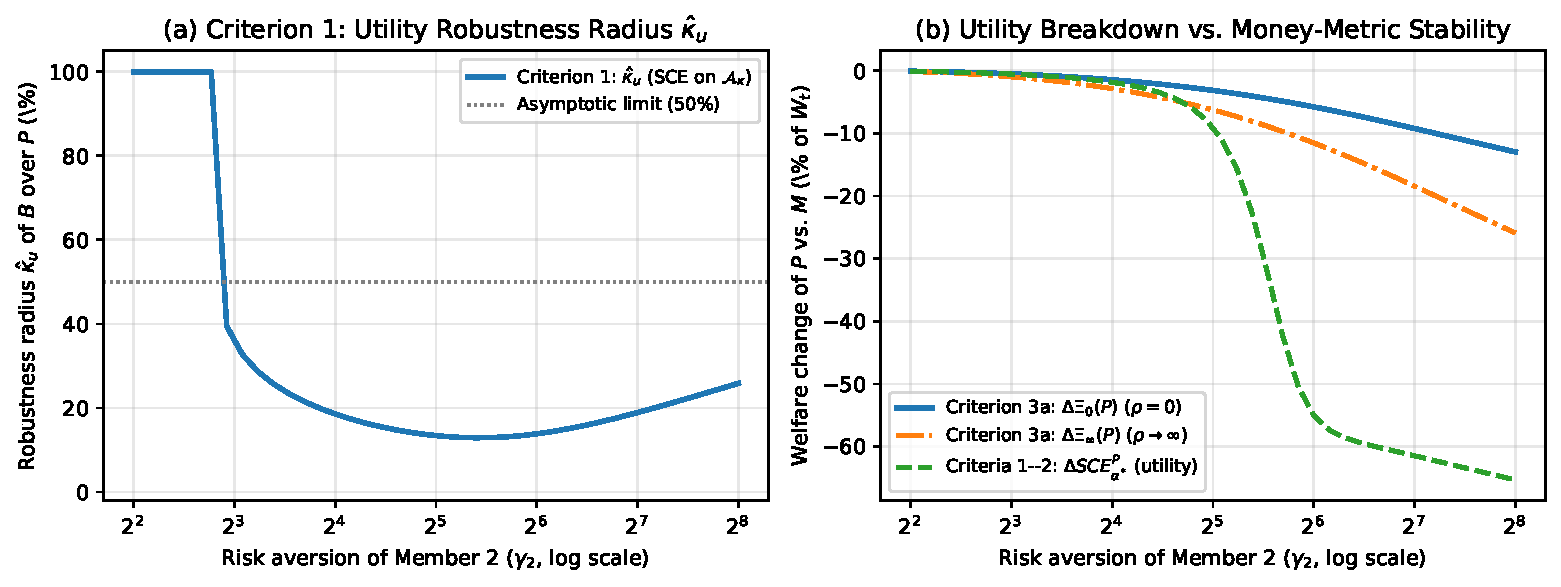
\includegraphics[width=\textwidth]{fig_sec9_gamma_grid.pdf}
  \caption{Sensitivity of Criterion 1 utility robustness radius ($\hat{\kappa}_u$) and Criteria 1, 2, and 3a welfare losses ($\Delta \Xi_0, \Delta \Xi_\infty, \Delta SCE_{\alpha^*}$) to $\gamma_2 \in [4, 256]$ (log scale, $\gamma_1 = 2$, Market A; for $\gamma_2 \le 4.3$, $B$ Pareto-dominates $P$).}
  \label{fig:sec9_gamma_grid}
\end{figure}

\subsubsection*{Part B: Synthesizing Criteria 1, 2, 3a, and 3b in the KT Pool under Transfers and Lotteries.}
To include the ex-post solidarity criterion $SCE_\rho^{\text{ep}}$ (Criterion 3b), which requires a common per-unit utility $v$, we return to the five-member heterogeneous-wealth KT pool of Section \ref{Sect:Het_Participants_Unique_Weights} in Market A ($W_i \in \{0.5, 0.75, 1.0, 1.5, 2.25\}$, $W_t = 6$). Alongside `Prop`, baseline `LEL-CE`, and `LEL-CE rand`, we evaluate a market-inconsistent rule, $\text{LEL-CE}(\tau = 1\%)$, which scales each member's baseline LEL-CE payoff by $(W_{i,t} + T_i)/W_{i,t}$ with $T_5 = -0.01 W_{5,t} = -0.0225$ ($-1.0\%$ of $W_{5,t}$), $T_1 = +0.0225$ ($+4.5\%$ of $W_{1,t}$), and $T_2 = T_3 = T_4 = 0$. Because $\pi_t(W_{i,t+1}^{\text{LEL-CE}}) = W_{i,t}$, this rule transfers exactly $0.0225$ of present market value from Member 5 to Member 1 while leaving Members 2, 3 and 4 unaffected. Under the homothetic reference-point scaling $\text{ref}_i(m_i) = (1+r)m_i$, each participant's equivalent-contribution ratio satisfies $m_i^k / W_{i,t} = CE_{i,t}^k / CE_{i,t}^{\text{AD}} = (CE_{i,t}^k / W_{i,t}) / y^{\text{AD}}$, where $y^{\text{AD}} = CE_{i,t}^{\text{AD}} / W_{i,t} = 1.03503$ is the common Global AD certainty-equivalent return in Market A. Both Criteria 3a and 3b are evaluated on the common grid $\rho \in \{0, 0.5\}$.

\begin{table}[!htbp]
  \centering
  \footnotesize
  \setlength{\tabcolsep}{2.8pt}
  \renewcommand{\arraystretch}{1.12}
  \caption{Part B: Comparison of deterministic, transfer-subsidized, and randomized rules in the Section \ref{Sect:Het_Participants_Unique_Weights} KT pool (Market A, changes relative to baseline LEL-CE in \% of $W_t$; individual columns in \% of $W_{i,t}$).}
  \label{tab:sec9_kt_synthesis}
  \begin{tabular*}{\textwidth}{@{\extracolsep{\fill}} l rr cr rrr rr @{}}
    \toprule
    & \multicolumn{2}{c}{Indiv.\ $\% \Delta CE_i$} 
    & \multicolumn{2}{c}{Criteria 1 \& 2} 
    & \multicolumn{3}{c}{Criterion 3a ($\Delta \Xi_\rho$)} 
    & \multicolumn{2}{c}{Criterion 3b ($\Delta SCE_\rho^{\text{ep}}$)} \\
    \cmidrule(lr){2-3} \cmidrule(lr){4-5} \cmidrule(lr){6-8} \cmidrule(l){9-10}
    Rule & Member 1 & Member 5 & Crit.\ 1 & $\Delta SCE_{\alpha^*}$ & $\rho{=}0$ & $\rho{=}0.5$ & $\rho{\to}\infty$ & $\rho{=}0$ & $\rho{=}0.5$ \\
    \midrule
    Prop                       & $-1.2077$ & $-1.2077$ & Pareto ($-$) & $-2.0166$ & $-1.1668$ & $-1.1668$ & $-1.1668$ & $-1.2077$ & $-1.2077$ \\
    LEL-CE (baseline)          & $\phantom{-}0.0000$  & $\phantom{-}0.0000$  & Base         & $\phantom{-}0.0000$  & $\phantom{-}0.0000$  & $\phantom{-}0.0000$  & $\phantom{-}0.0000$  & $\phantom{-}0.0000$  & $\phantom{-}0.0000$  \\
    LEL-CE ($\tau = 1\%$ sub.) & $\phantom{-}4.8935$  & $-0.7564$ & Trade-off    & $-0.2366$ & $\phantom{-}0.1199$  & $\phantom{-}0.1099$  & $-0.7308$ & $\phantom{-}0.0000$  & $-0.0047$ \\
    LEL-CE rand                & $\phantom{-}0.1682$  & $\phantom{-}0.1682$  & Pareto ($+$) & $\phantom{-}0.1682$  & $\phantom{-}0.1626$  & $\phantom{-}0.1626$  & $\phantom{-}0.1626$  & $\phantom{-}0.0000$  & $-0.2000$ \\
    \bottomrule
  \end{tabular*}
\end{table}

Table \ref{tab:sec9_kt_synthesis} shows how Criteria 3a and 3b jointly capture cross-sectional transfers and intra-state lotteries:
\begin{itemize}
    \item \textbf{Constant proportionality factor $y^{\text{AD}} = 1.03503$:}
    
    For homothetic rules (`Prop` and `LEL-CE rand`), $\Delta \Xi_\rho(k)$ is independent of $\rho$ and equals the time-$(t+1)$ efficiency gain divided by $y^{\text{AD}} = 1.03503$ ($-1.2077\% / 1.03503 = -1.1668\%$ and $+0.1682\% / 1.03503 = +0.1626\%$), converting time-$(t+1)$ certainty equivalents into time-$t$ equivalent contributions;
    \item \textbf{Subsidized LEL-CE ($\tau = 1\%$):} 
    
    Because each member's LEL-CE payoff is scaled by $(W_{i,t} + T_i)/W_{i,t}$, Members 2, 3 and 4 are unaffected ($\Delta CE_2 = \Delta CE_3 = \Delta CE_4 = 0$), while Member 1 gains $+4.8935\%$ and Member 5 loses $-0.7564\%$. As we can see Criterion 2 leads to an overall fund welfare loss of $-0.2366\%$, while for small value of $\rho$ we get a fund gain of about 0.10\%, which reverses for larger values of inequality aversion;
    \item \textbf{Randomized LEL-CE (`LEL-CE rand`):} 
    
    Every ex-ante criterion (Criteria 1, 2, and 3a for all $\rho \ge 0$) ranks `LEL-CE rand` strictly above `LEL-CE`, whereas the ex-post criterion $SCE_\rho^{\text{ep}}$ (Criterion 3b) strips out the lottery gain at $\rho = 0$ ($0.0000\%$) and reverses the ranking to $-0.2000\%$ at $\rho = 0.5$.
\end{itemize}
